% =============================================================================
% Brouillon de rapport organise autour du Pivot C : le diagnostic du dataset
% devient le coeur du rapport plutot que d'essayer de "sauver" la performance.
%
% Sections marquees [TODO] ou [A COMPLETER] sont des squelettes a remplir.
% La section "Diagnostic du dataset" est ecrite integralement avec les chiffres
% et les figures generees par code/diagnostic_signal.py, code/diagnostic_figures.py
% et code/diagnostic_regression.py.
%
% Les figures sont supposees dans graphs/ (01_loss_distribution.png, etc.).
% =============================================================================

\documentclass[a4paper,12pt]{article}

\usepackage[utf8]{inputenc}
\usepackage[T1]{fontenc}
\usepackage[french]{babel}
\usepackage{graphicx}
\usepackage{booktabs}
\usepackage{array}
\usepackage{caption}
\usepackage{hyperref}
\usepackage{geometry}
\geometry{margin=2.5cm}

\title{Diagnostic d'un dataset synth\'etique pour la d\'etection d'incidents \`a fort impact financier\\
\large Une approche m\'ethodologique appliqu\'ee \`a un dataset Kaggle de cybers\'ecurit\'e}
\author{
Noa ISABEY \\
L\'eo PROSPER \\
Ashkan MIRI \\
Steve KINGSLEY ARULNEASATHAS
}
\date{April 2026}

\begin{document}

\maketitle
\tableofcontents
\newpage

% =============================================================================
\section{Introduction}
% =============================================================================

\textbf{[A COMPLETER]} Ce rapport pr\'esente notre travail sur le projet de Machine Learning du semestre~6, dont l'objectif initial est de pr\'edire les incidents de cybers\'ecurit\'e \`a \emph{fort impact financier} \`a partir d'un jeu de donn\'ees public.

Nous avons retenu le dataset \emph{Global Cybersecurity Threats 2015-2024} disponible sur Kaggle, qui contient 3000 incidents d\'ecrits par 10 colonnes (pays, ann\'ee, type d'attaque, industrie cibl\'ee, perte financi\`ere, nombre d'utilisateurs affect\'es, source de l'attaque, type de vuln\'erabilit\'e, m\'ecanisme de d\'efense utilis\'e, temps de r\'esolution).

Nous d\'efinissons la t\^ache comme une \textbf{classification binaire}: pr\'edire si la perte financi\`ere d\'epasse le quantile~0.75 de la distribution observ\'ee, soit \texttt{Financial Loss} $\geq$ 75.63 M\$.

\textbf{Plan du rapport.} La section~\ref{sec:methodo} d\'ecrit notre m\'ethodologie. La section~\ref{sec:results} pr\'esente les r\'esultats des mod\`eles candidats. La section~\ref{sec:diagnostic} constitue le c\oe ur de notre travail: face \`a une convergence des mod\`eles autour d'une F1 macro de 0.49 et d'un AUC de 0.5, nous avons men\'e un diagnostic statistique du dataset pour identifier l'origine de cette performance plate. La section~\ref{sec:discussion} en tire les enseignements m\'ethodologiques.

% =============================================================================
\section{M\'ethodologie}
\label{sec:methodo}
% =============================================================================

\subsection{Pr\'etraitement des donn\'ees}

Notre pipeline de pr\'etraitement (\texttt{code/preprocess.py}) applique:
\begin{itemize}
  \item normalisation des valeurs textuelles \emph{Unknown}, \emph{N/A}, \emph{none} en une cat\'egorie unique \texttt{Unknown};
  \item conversion explicite en types num\'eriques pour \texttt{Year}, \texttt{Financial Loss}, \texttt{Number of Affected Users}, \texttt{Incident Resolution Time};
  \item rapport de qualit\'e des donn\'ees (doublons, valeurs manquantes, cardinalit\'e cat\'egorielle).
\end{itemize}

L'ex\'ecution sur notre dataset (3000 lignes, 10 colonnes) ne r\'ev\`ele aucun doublon, aucune valeur manquante apr\`es normalisation, et 768 valeurs \texttt{Unknown} concentr\'ees sur \texttt{Attack Source} (~25\%). Les cardinalit\'es cat\'egorielles sont mod\'er\'ees: \texttt{Country}=10, \texttt{Attack Type}=6, \texttt{Target Industry}=7, \texttt{Attack Source}=4, \texttt{Security Vulnerability Type}=4, \texttt{Defense Mechanism Used}=5.

\subsection{Construction de la cible}

Nous d\'erivons une cible binaire \texttt{High Financial Impact} en seuillant \texttt{Financial Loss} au quantile~0.75 (75.63~M\$). Le ratio de classes obtenu est 75/25 par construction (2249 incidents en classe~0, 751 en classe~1).

\subsection{Mod\`eles candidats}

Nous comparons quatre mod\`eles couvrant un spectre de complexit\'es:
\begin{itemize}
  \item \textbf{Baseline} (\texttt{DummyClassifier(strategy="most\_frequent")}): plancher de r\'ef\'erence;
  \item \textbf{Logistic Regression}: mod\`ele lin\'eaire, sensible \`a la mise \`a l'\'echelle;
  \item \textbf{Decision Tree}: capture des effets non-lin\'eaires et des interactions;
  \item \textbf{Random Forest}: agr\'egation d'arbres, robuste au bruit.
\end{itemize}

Tous les mod\`eles non-triviaux sont s\'electionn\'es par \texttt{GridSearchCV} avec validation crois\'ee \texttt{StratifiedKFold(n\_splits=5)}, scoring F1 sur la classe positive. \texttt{class\_weight="balanced"} est utilis\'e syst\'ematiquement pour compenser le d\'es\'equilibre 75/25.

\subsection{M\'etriques d'\'evaluation}

Nous rapportons l'accuracy, la pr\'ecision, le rappel et la F1 macro (qui pond\`ere \'egalement les deux classes), ainsi que le ROC-AUC \emph{One-vs-Rest}. La F1 macro est notre m\'etrique principale car le d\'es\'equilibre rend l'accuracy trompeuse: pr\'edire toujours la classe majoritaire donne 75\% d'accuracy mais une F1 macro de 0.43.

% =============================================================================
\section{R\'esultats exp\'erimentaux}
\label{sec:results}
% =============================================================================

\subsection{Performance des mod\`eles}

Le tableau~\ref{tab:results} r\'esume les performances obtenues sur l'ensemble de test (900 \'echantillons, 30\% du dataset).

\begin{table}[h!]
\centering
\caption{Performance des mod\`eles sur l'ensemble de test (900 \'echantillons). L'\'ecart train/test indique la qualit\'e de g\'en\'eralisation: un \'ecart \'elev\'e signale un sur-apprentissage.}
\label{tab:results}
\begin{tabular}{lrrrrr}
\toprule
\textbf{Mod\`ele} & \textbf{Train F1} & \textbf{Test F1} & \textbf{Accuracy} & \textbf{ROC-AUC} & \textbf{Train$-$Test} \\
\midrule
Baseline (most freq.) & 0.4284 & 0.4286 & 0.7500 & 0.500 & $-0.000$ \\
Logistic Regression   & 0.5248 & 0.4775 & 0.5256 & 0.498 & $+0.047$ \\
Decision Tree         & 0.6509 & 0.4828 & 0.5089 & 0.524 & $+0.168$ \\
Random Forest         & 0.9095 & 0.4914 & 0.7033 & 0.505 & $+0.418$ \\
\bottomrule
\end{tabular}
\end{table}

\subsection{Constat: convergence des mod\`eles autour de l'al\'eatoire}

Trois observations s'imposent:

\begin{enumerate}
  \item Tous les mod\`eles non-triviaux convergent vers une F1 macro de l'ordre de 0.48-0.49, l\'eg\`erement au-dessus de la baseline majoritaire (0.43) mais loin de toute performance utilisable en pratique.
  \item Les ROC-AUC sont tous proches de 0.50, c'est-\`a-dire \emph{au niveau du hasard} pour un classifieur binaire.
  \item Le Random Forest pr\'esente un \'ecart train/test consid\'erable ($0.91 \rightarrow 0.49$), \emph{visible sur la figure~\ref{fig:overfit}}, signe que le mod\`ele dispose d'une capacit\'e suffisante pour m\'emoriser l'ensemble d'entra\^inement mais ne parvient pas \`a g\'en\'eraliser.
\end{enumerate}

\begin{figure}[h!]
\centering
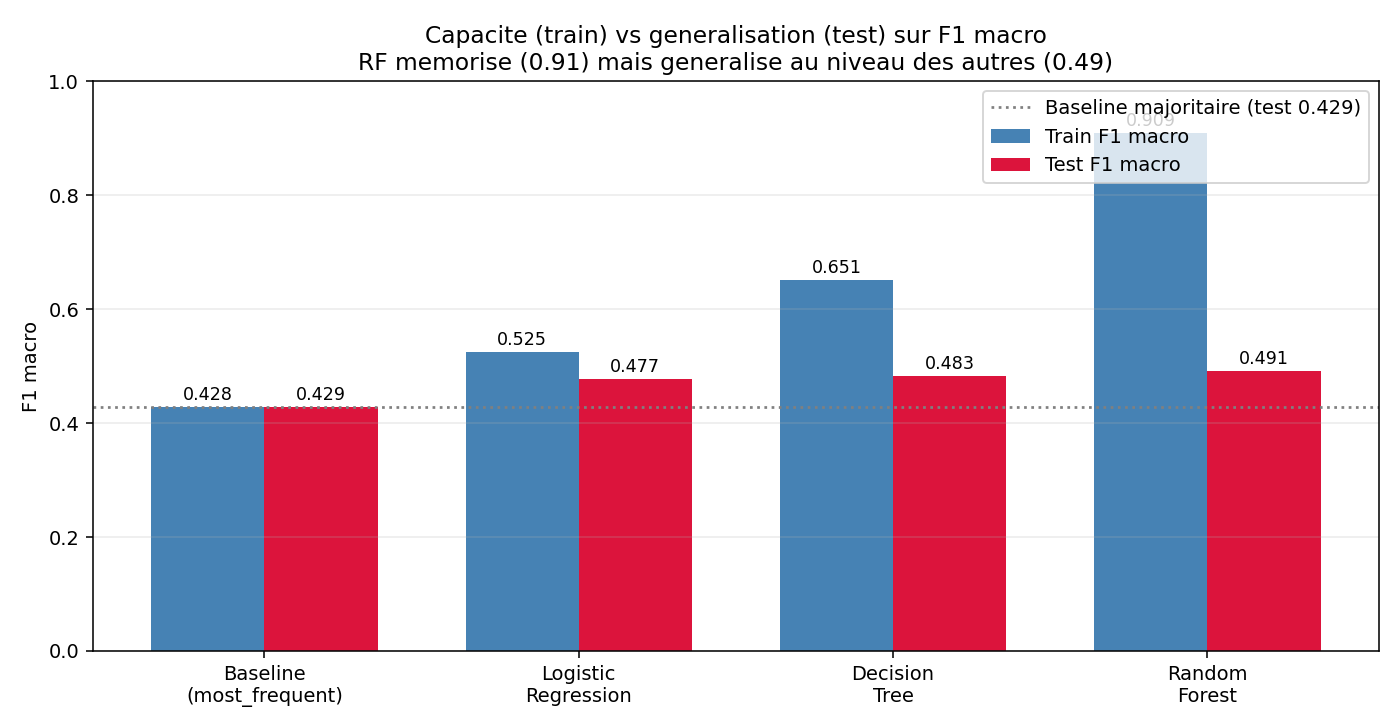
\includegraphics[width=0.95\linewidth]{graphs/05_train_vs_test_overfit.png}
\caption{Comparaison F1 macro train vs test pour chaque mod\`ele. Le Random Forest m\'emorise (train 0.91) mais g\'en\'eralise au m\^eme niveau que les autres mod\`eles (test 0.49), peine au-dessus de la baseline majoritaire (0.43).}
\label{fig:overfit}
\end{figure}

Cette signature (capacit\'e suffisante + g\'en\'eralisation au niveau du hasard) sugg\`ere que le probl\`eme n'est pas du c\^ot\'e du mod\`ele mais du c\^ot\'e des \emph{donn\'ees}: il n'y aurait simplement \emph{pas de signal exploitable} dans les features pour pr\'edire la cible. C'est l'hypoth\`ese que la section suivante teste rigoureusement.

% =============================================================================
\section{Diagnostic du dataset}
\label{sec:diagnostic}
% =============================================================================

\subsection{Quatre hypoth\`eses \`a tester}

Devant une performance plate sur trois familles de mod\`eles diff\'erentes, nous formulons quatre hypoth\`eses concurrentes pour expliquer ce r\'esultat:

\begin{description}
  \item[H1 -- Capacit\'e insuffisante des mod\`eles.] Les algorithmes ne seraient pas assez expressifs pour capturer la relation features $\rightarrow$ cible.
  \item[H2 -- Pr\'eprocessing inadapt\'e.] Notre pipeline d\'etruirait l'information pertinente (encodage, scaling, etc.).
  \item[H3 -- Features individuellement non-informatives.] Aucune feature ne porterait, prise s\'epar\'ement, d'information sur la cible.
  \item[H4 -- Dataset structurellement al\'eatoire.] La cible serait ind\'ependante des features par construction du dataset.
\end{description}

Notons que H1 et H2 \emph{sont d\'ej\`a partiellement r\'efut\'ees} par les r\'esultats de la section pr\'ec\'edente: le Random Forest non-lin\'eaire dispose visiblement de la capacit\'e n\'ecessaire (train F1 = 0.91), et notre pipeline est l'application standard des bonnes pratiques sklearn. Nous validons cependant H3 et H4 explicitement.

\subsection{H3 -- Mutual information sur les variables num\'eriques}

Nous calculons la \emph{mutual information} entre chaque variable num\'erique (hors target et hors \texttt{Financial Loss} dont la target d\'erive) et la cible binaire. Le tableau~\ref{tab:mi} et la figure~\ref{fig:mi} pr\'esentent les r\'esultats.

\begin{table}[h!]
\centering
\caption{Mutual information entre features num\'eriques et la cible.}
\label{tab:mi}
\begin{tabular}{lr}
\toprule
\textbf{Feature} & \textbf{Mutual Information} \\
\midrule
Incident Resolution Time (in Hours) & 0.006326 \\
Year                                 & 0.000000 \\
Number of Affected Users             & 0.000000 \\
\bottomrule
\end{tabular}
\end{table}

\begin{figure}[h!]
\centering
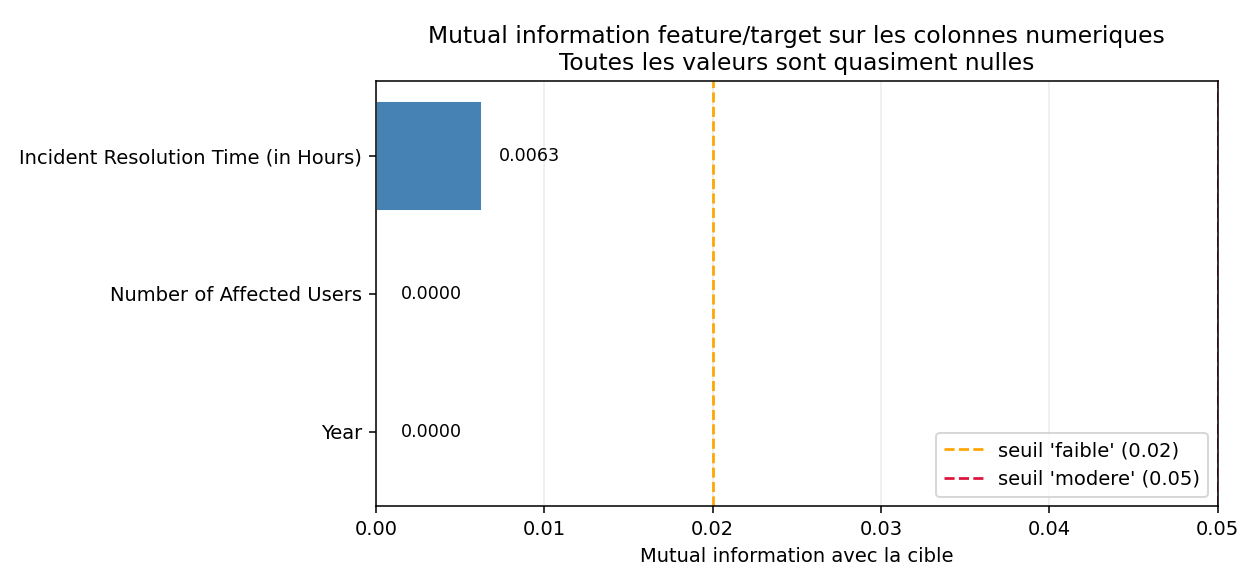
\includegraphics[width=0.85\linewidth]{graphs/02_mutual_info_numeric.png}
\caption{Mutual information entre les variables num\'eriques et la cible. Les valeurs sont toutes en de\c{c}\`a du seuil de 0.02 conventionnellement consid\'er\'e comme tr\`es faible.}
\label{fig:mi}
\end{figure}

\textbf{Interpr\'etation.} Une MI de 0 signifie que la connaissance de la feature n'apporte litt\'eralement aucune r\'eduction d'incertitude sur la cible. Sur les trois features num\'eriques disponibles, deux sont \`a 0 exactement (\texttt{Year} et \texttt{Number of Affected Users}), la troisi\`eme est \`a 0.006 (largement en dessous des seuils 0.02-0.05 utilis\'es comme rep\`eres dans la litt\'erature). H3 est confirm\'ee.

\subsection{H3 -- Cram\'er's V et chi$^2$ sur les variables cat\'egorielles}

Pour chaque variable cat\'egorielle, nous calculons la statistique \emph{Cram\'er's V} (chi$^2$ de Pearson normalis\'e dans $[0, 1]$) ainsi que la p-value du test du chi$^2$ d'ind\'ependance. Les r\'esultats figurent dans le tableau~\ref{tab:cramers} et la figure~\ref{fig:cramers}.

\begin{table}[h!]
\centering
\caption{Cram\'er's V et test du chi$^2$ entre features cat\'egorielles et cible.}
\label{tab:cramers}
\begin{tabular}{lrrr}
\toprule
\textbf{Feature} & \textbf{Modalit\'es} & \textbf{Cram\'er's V} & \textbf{$\chi^2$ p-value} \\
\midrule
Country                       & 10 & 0.058 & 0.343 \\
Attack Type                   & 6  & 0.042 & 0.376 \\
Target Industry               & 7  & 0.034 & 0.751 \\
Defense Mechanism Used        & 5  & 0.033 & 0.516 \\
Security Vulnerability Type   & 4  & 0.028 & 0.494 \\
Attack Source                 & 4  & 0.026 & 0.561 \\
\bottomrule
\end{tabular}
\end{table}

\begin{figure}[h!]
\centering
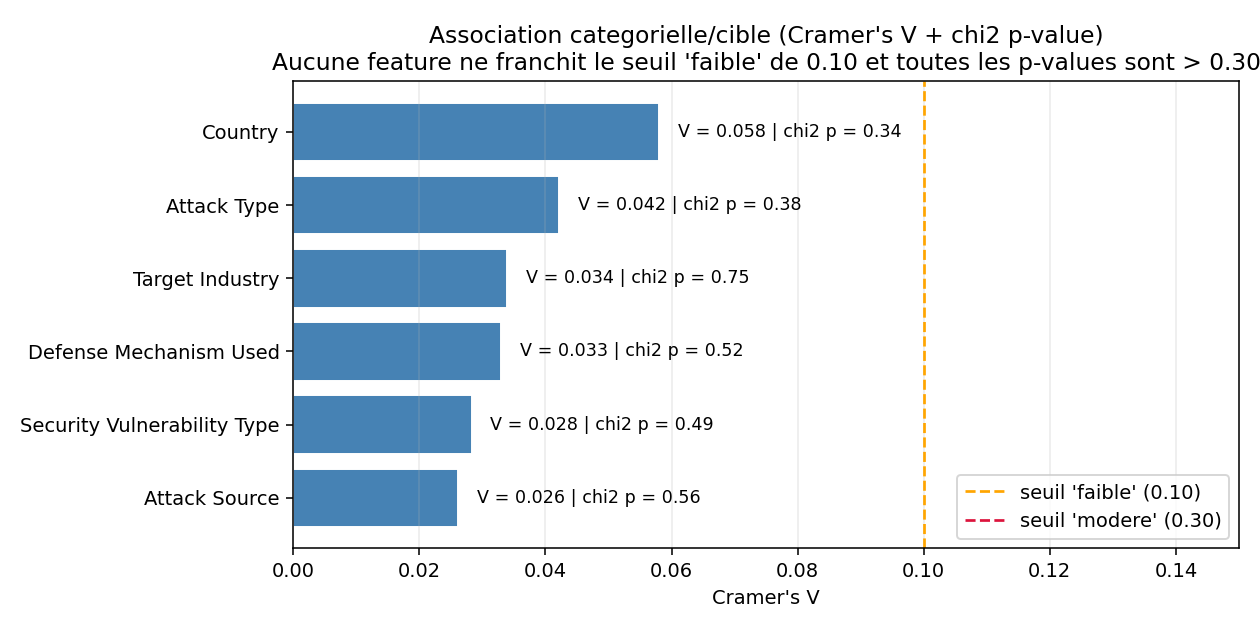
\includegraphics[width=0.85\linewidth]{graphs/03_cramers_v_categorical.png}
\caption{Cram\'er's V et p-value du test du chi$^2$ pour chaque variable cat\'egorielle. Aucune feature ne franchit le seuil de 0.10 (association \og faible \fg) et toutes les p-values sont sup\'erieures \`a 0.30.}
\label{fig:cramers}
\end{figure}

\textbf{Interpr\'etation.} Le seuil conventionnel de Cram\'er's V est 0.10 pour qualifier une association de \og faible \fg, 0.30 pour \og mod\'er\'ee \fg. Aucune de nos six variables cat\'egorielles ne franchit le seuil de 0.10. De plus, aucune p-value du test du chi$^2$ n'est inf\'erieure \`a 0.30: nous ne pouvons rejeter l'hypoth\`ese d'ind\'ependance pour aucune feature au seuil $\alpha = 0.05$. La feature la plus \og prometteuse \fg{} (\texttt{Country}, $V = 0.058$, $p = 0.34$) reste statistiquement non-discriminante.

Pour rendre cette absence d'association visualisable, la figure~\ref{fig:posrate} repr\'esente, pour les trois variables cat\'egorielles ayant le plus haut Cram\'er's V, le taux de classe~1 par modalit\'e accompagn\'e d'un intervalle de confiance \`a 95\% (formule de Wald).

\begin{figure}[h!]
\centering
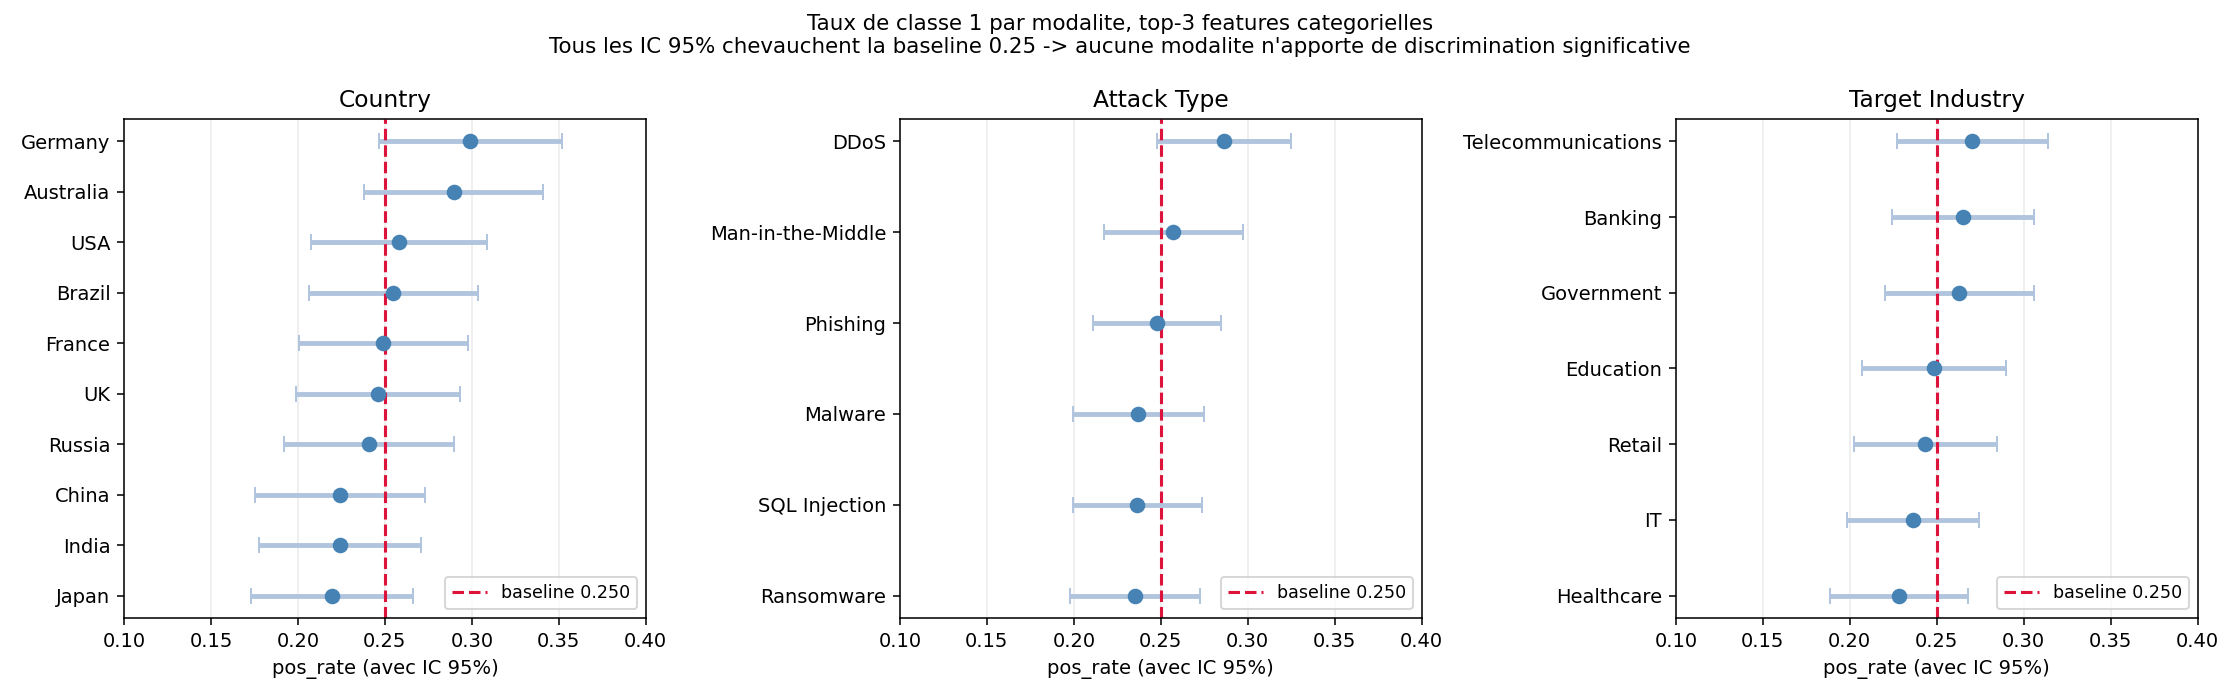
\includegraphics[width=\linewidth]{graphs/04_pos_rate_top_categories.png}
\caption{Taux de classe~1 (\og High Financial Impact \fg) par modalit\'e pour les trois variables cat\'egorielles ayant le Cram\'er's V le plus \'elev\'e. Tous les intervalles de confiance \`a 95\% chevauchent la baseline globale 0.25, confirmant qu'aucune modalit\'e ne discrimine significativement.}
\label{fig:posrate}
\end{figure}

\subsection{H4 -- Distribution de Financial Loss}

L'absence de signal sur les autres colonnes nous a conduits \`a examiner la distribution de la variable d'origine \texttt{Financial Loss} \`a partir de laquelle la cible est construite. La figure~\ref{fig:loss} pr\'esente l'histogramme observ\'e accompagn\'e de la densit\'e th\'eorique d'une loi uniforme sur $[0.50, 99.99]$.

\begin{figure}[h!]
\centering
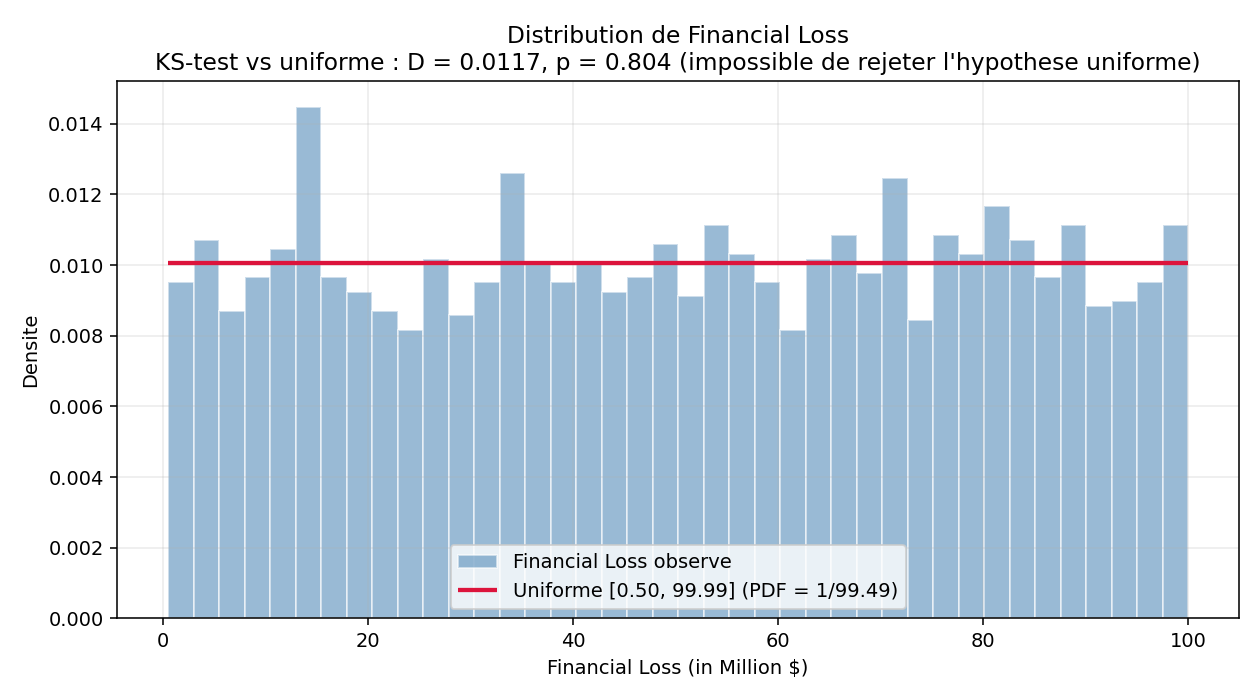
\includegraphics[width=0.95\linewidth]{graphs/01_loss_distribution.png}
\caption{Distribution de \texttt{Financial Loss} (3000 incidents). La densit\'e observ\'ee suit visuellement une loi uniforme sur $[0.50, 99.99]$. Le test de Kolmogorov-Smirnov contre cette uniforme donne $D = 0.012$ et $p = 0.804$: l'hypoth\`ese d'uniformit\'e ne peut pas \^etre rejet\'ee.}
\label{fig:loss}
\end{figure}

\textbf{Statistiques observ\'ees vs uniforme th\'eorique.} La moyenne empirique est 50.49, la m\'ediane 50.80, l'\'ecart-type 28.79 -- exactement les valeurs attendues pour une uniforme sur $[0.5, 100]$ dont l'\'ecart-type th\'eorique est $99.5/\sqrt{12} \approx 28.72$. Le test de Kolmogorov-Smirnov contre cette uniforme donne $D = 0.0117$, $p = 0.804$: \textbf{l'hypoth\`ese que \texttt{Financial Loss} suit une loi uniforme aleatoire ne peut pas \^etre rejet\'ee.}

\subsection{Validation par r\'egression directe}

Une derni\`ere objection serait que la binarisation au quantile~0.75 d\'etruit un signal qui existerait dans la valeur continue de \texttt{Financial Loss}. Nous testons cette hypoth\`ese en r\'egressant directement la valeur continue (cf. \texttt{code/diagnostic\_regression.py}). Le tableau~\ref{tab:regression} pr\'esente les r\'esultats.

\begin{table}[h!]
\centering
\caption{R\'egression directe de \texttt{Financial Loss} (M\$). Test set de 30\% (900 \'echantillons).}
\label{tab:regression}
\begin{tabular}{lrrrrr}
\toprule
\textbf{Mod\`ele} & \textbf{Train R$^2$} & \textbf{Test R$^2$} & \textbf{Train MAE} & \textbf{Test MAE} & \textbf{Test RMSE} \\
\midrule
Dummy (mean)              &  0.000 &  $-$0.000 & 25.06 & 24.77 & 28.63 \\
Linear Regression         &  0.017 &  $-$0.017 & 24.75 & 24.92 & 28.88 \\
Random Forest ($n=200$)   &  0.855 &  $-$0.034 &  9.42 & 25.06 & 29.11 \\
\bottomrule
\end{tabular}
\end{table}

\textbf{Interpr\'etation.} Le R$^2$ test est \emph{n\'egatif} pour la r\'egression lin\'eaire et le Random Forest. Un R$^2$ n\'egatif signifie que les pr\'edictions du mod\`ele sont \emph{statistiquement pires} que celles d'un mod\`ele constant pr\'edisant la moyenne du train. Le RF affiche par ailleurs un \'ecart train/test consid\'erable (R$^2$ train de 0.855 vs test de $-0.034$): m\^eme constatation que pour la classification, le mod\`ele a la capacit\'e de m\'emoriser l'ensemble d'entra\^inement mais rien \`a g\'en\'eraliser.

Cette section verrouille H4: ce n'est pas la binarisation qui d\'etruit le signal, le signal n'existe \emph{simplement pas} dans le dataset, sous quelque forme que ce soit.

\subsection{Synth\`ese du diagnostic}

L'ensemble des tests converge vers une m\^eme conclusion: le dataset \emph{Global Cybersecurity Threats 2015-2024} se comporte, pour la t\^ache que nous avons consid\'er\'ee, comme un \textbf{tirage al\'eatoire ind\'ependant}.

\begin{itemize}
  \item \texttt{Financial Loss} suit une loi uniforme sur $[0.5, 100]$ ($p = 0.80$ pour le test KS), ce qui est typique d'un \emph{dataset synth\'etique} g\'en\'er\'e par tirage uniforme plut\^ot qu'observ\'e.
  \item Aucune feature num\'erique ne porte de mutual information mesurable avec la cible (max~0.006).
  \item Aucune feature cat\'egorielle ne pr\'esente d'association significative avec la cible (Cram\'er's V $\leq 0.058$, p-value $\chi^2 \geq 0.34$).
  \item La r\'egression directe sur la valeur continue ne fait pas mieux: R$^2$ test n\'egatif sur LR et RF.
\end{itemize}

Aucun mod\`ele de Machine Learning, ind\'ependamment de sa complexit\'e, ne peut \emph{en principe} d\'epasser la baseline majoritaire sur ce dataset pour cette t\^ache: il n'y a aucune information \`a apprendre.

% =============================================================================
\section{Discussion}
\label{sec:discussion}
% =============================================================================

\subsection{Apprentissages m\'ethodologiques}

Notre travail illustre une comp\'etence souvent peu enseign\'ee mais essentielle en pratique: \textbf{savoir reconna\^itre quand le Machine Learning n'est pas le bon outil}. Une performance plate sur plusieurs mod\`eles n'est pas une fatalit\'e \`a accepter ni un signal qu'il faut ajouter des features ou augmenter la capacit\'e: c'est un signal qu'il faut investiguer.

L'instrumentation diagnostique mise en place (KS-test, mutual information, Cram\'er's V, chi$^2$, intervalles de confiance par modalit\'e, r\'egression de v\'erification) est r\'eutilisable telle quelle sur tout futur dataset et constitue un \og kit de diagnostic \fg{} avant de se lancer dans le tuning d'hyperparam\`etres.

\subsection{Conditions pour rendre la t\^ache faisable}

Notre pipeline est volontairement \emph{dataset-agnostic}: \texttt{preprocess.py} et \texttt{training\_comparison.py} acceptent n'importe quel CSV avec des colonnes num\'eriques et cat\'egorielles et s'adaptent automatiquement. Pour appliquer la m\^eme m\'ethodologie \`a un dataset porteur de signal, il suffirait de:
\begin{itemize}
  \item s\'electionner un dataset r\'eel (plut\^ot que synth\'etique) -- des candidats reconnus pour la d\'etection d'intrusion existent (NSL-KDD, UNSW-NB15, CICIDS2017);
  \item appliquer le m\^eme \texttt{diagnostic\_signal.py} en pr\'eambule pour confirmer la pr\'esence de signal;
  \item ex\'ecuter le m\^eme \texttt{training\_comparison.py} pour comparer les mod\`eles.
\end{itemize}

\subsection{Limites de notre \'etude}

Notre conclusion porte sur la t\^ache sp\'ecifique de pr\'ediction de \emph{High Financial Impact} sur \emph{ce} dataset. Il reste possible que d'autres formulations (clustering non-supervis\'e, d\'etection d'anomalies sur une sous-population sp\'ecifique) r\'ev\`elent des structures que nous n'avons pas cherch\'ees. Notre travail valide n\'eanmoins que la t\^ache de classification supervis\'ee initialement choisie est intrins\`equement infaisable.

% =============================================================================
\section{Conclusion}
% =============================================================================

Nous avons appliqu\'e \`a un dataset Kaggle de cybers\'ecurit\'e une cha\^ine de Machine Learning standard (pr\'eprocessing, ing\'enierie de features, comparaison de mod\`eles, validation crois\'ee, tuning d'hyperparam\`etres). Face \`a une convergence des trois familles de mod\`eles vers un AUC de 0.5, nous n'avons pas tent\'e d'optimiser des chiffres sans signification mais avons men\'e un \textbf{diagnostic statistique rigoureux}, qui d\'emontre que le dataset ne porte aucun signal exploitable pour la t\^ache choisie.

Ce r\'esultat est, en soi, une contribution m\'ethodologique: identifier qu'un probl\`eme est \emph{structurellement infaisable} \`a partir des donn\'ees disponibles est une comp\'etence aussi importante qu'optimiser un mod\`ele lorsque c'est possible. Notre pipeline diagnostic est r\'eutilisable et notre pipeline de mod\'elisation est pr\^et \`a \^etre appliqu\'e \`a tout dataset porteur de signal.

% =============================================================================
\appendix
\section*{Annexe -- Reproductibilit\'e}
\addcontentsline{toc}{section}{Annexe -- Reproductibilit\'e}
% =============================================================================

\begin{itemize}
  \item Construction de la cible et entra\^inement initial: \texttt{python code/main.py} (depuis la racine du projet)
  \item Diagnostic statistique chiffr\'e: \texttt{python code/diagnostic\_signal.py}
  \item G\'en\'eration des figures du rapport: \texttt{python code/diagnostic\_figures.py} (sortie dans \texttt{graphs/})
  \item Diagnostic compl\'ementaire en r\'egression: \texttt{python code/diagnostic\_regression.py}
  \item Compilation du rapport: \texttt{pdflatex rapport.tex}; nettoyage des artefacts via \texttt{make clean}
\end{itemize}

\end{document}
